\section{Limitations and future work}
\label{sec:limit}
\subsection{Broader context in user privacy concerns}
Privacy is a critical aspect of LLM personalization in the real world. In our setting, we personalize responses based on only preferences and activities shared by the user in previous user-chatbot interactions, and the model uses this information for its own responses without external sharing. To avoid potential privacy risks associated with real user data, we intentionally propose a synthetic data curation pipeline in this work. This synthetic approach allows researchers in the community to safely explore personalization methods. One possible direction for future work could be designing question-answer pairs that specifically involve sensitive user information.

\subsection{More advanced retrieval methods}
Our current exploration of retrieval-augmented methods, such as RAG and Mem0, is intended as a proof of concept, as the primary focus of this work is on the design and release of the personalization benchmark. We are excited to encourage more exploration on state-of-the-art long-context, memory, and retrieval-augmented generation methods in future work, especially those that preserve and understand the evolution of user personas and reasons behind preference updates, as well as enhancing user personalization in new or unseen scenarios.

\subsection{Potential artifacts in the synthetic data generation process}
To reduce artifacts that might make the benchmark artificially easier, we've taken several steps. For example, we removed question-answer pairs where the correct answer was unintentionally obvious, such as being noticeably longer or sharing identical key words with the questions. We also filtered out queries that an LLM can answer correctly more than once in three attempts, without seeing any actual conversation context. Besides, we have included checks in our human evaluations to confirm that the correct answers can indeed be derived from the provided context.

\subsection{Potential gaps between evaluations on open-ended generations and multiple choices}
In purely open-ended generative settings, personalization can lead to many possible correct answers, depending on how the user persona is used and which related user preference is used. Meanwhile, open-ended evaluations are computationally expensive due to the need for LLM-as-a-Judge for each question-answer pair. As a result, we evaluate generative tasks by computing the joint log-likelihood of each candidate option, without explicitly presenting all four options in the prompt. This approach yields similar patterns with those observed in standard discriminative evaluations in our experiment, while offering a more reliable basis for benchmarking performance compared to fully open-ended ones.


\newpage

\FloatBarrier

\section{Details on Human Evaluation}
\label{sec:human_eval}


The purpose of the human evaluation study is to validate the overall quality of the generation process described in \S~\ref{sec:curation}. Note that we are not asking for human performance on the questions, given the intractability of reading the long contexts. Instead, we provide evaluators with the questions and answers, as well as the conversations and meta-data that they are grounded in.

We use the potato package~\citep{pei2022potato} for implementation of the interface. A screenshot is shown in Figure~\ref{fig:eval_interface}.
For each entry, we ask for True/False evaluations on 4 dimensions:
\begin{enumerate}
    \item Appropriateness: The question is well-formed and corresponds to the type.
    \item Relevance: The question is relevant to the conversation and persona.
    \item Correctness: `Correct\_Response' is indeed correct, and can be derived from the context.
    \item Best Response: `Correct\_Response' is better than all of the `Incorrect\_Responses.'
\end{enumerate}

We recruited three authors from among the authors of this work.\footnote{We recognize that the authors may not be fully impartial annotators. To reduce this issue, the three authors who participated were not directly involved with the data generation process. We nevertheless will consider external annotators for future work.} We iterated the annotation instructions and template with active feedback from the annotators, leading to the finalized version.

We selected 90 entries (18 topics * 5 randomly sampled questions each) for annotation.  To ease annotator mental load, all entries come from a single persona. Each entry is annotated 3 times, and we assign the majority class label.  Each task took about 1.5 minutes to complete. 

For each entry and each dimension, we calculate the proportion of `True', as well as We calculate inter-rater reliability with Gwet's AC1~\citep{gwet2008computing}. We use this metric as it accounts for the heavy class imbalance towards True. 
Considering the results, 97.8\% of entries were rated as appropriate (AC1=0.928), 95.6\% as relevance (AC1=0.899), 97.8\% as correct (AC1=0.877), and 90\% as being the best response (AC1=0.560). All proportions are over 90\%, and agreement is very high for dimensions 1,2, and 3, and moderate for dimension 4 (likely because it is subjective). Given this small-scale human evaluation, we can conclude that the generation quality of~\datasetname~is quite reasonable. 


\begin{figure}[h]
    \centering
    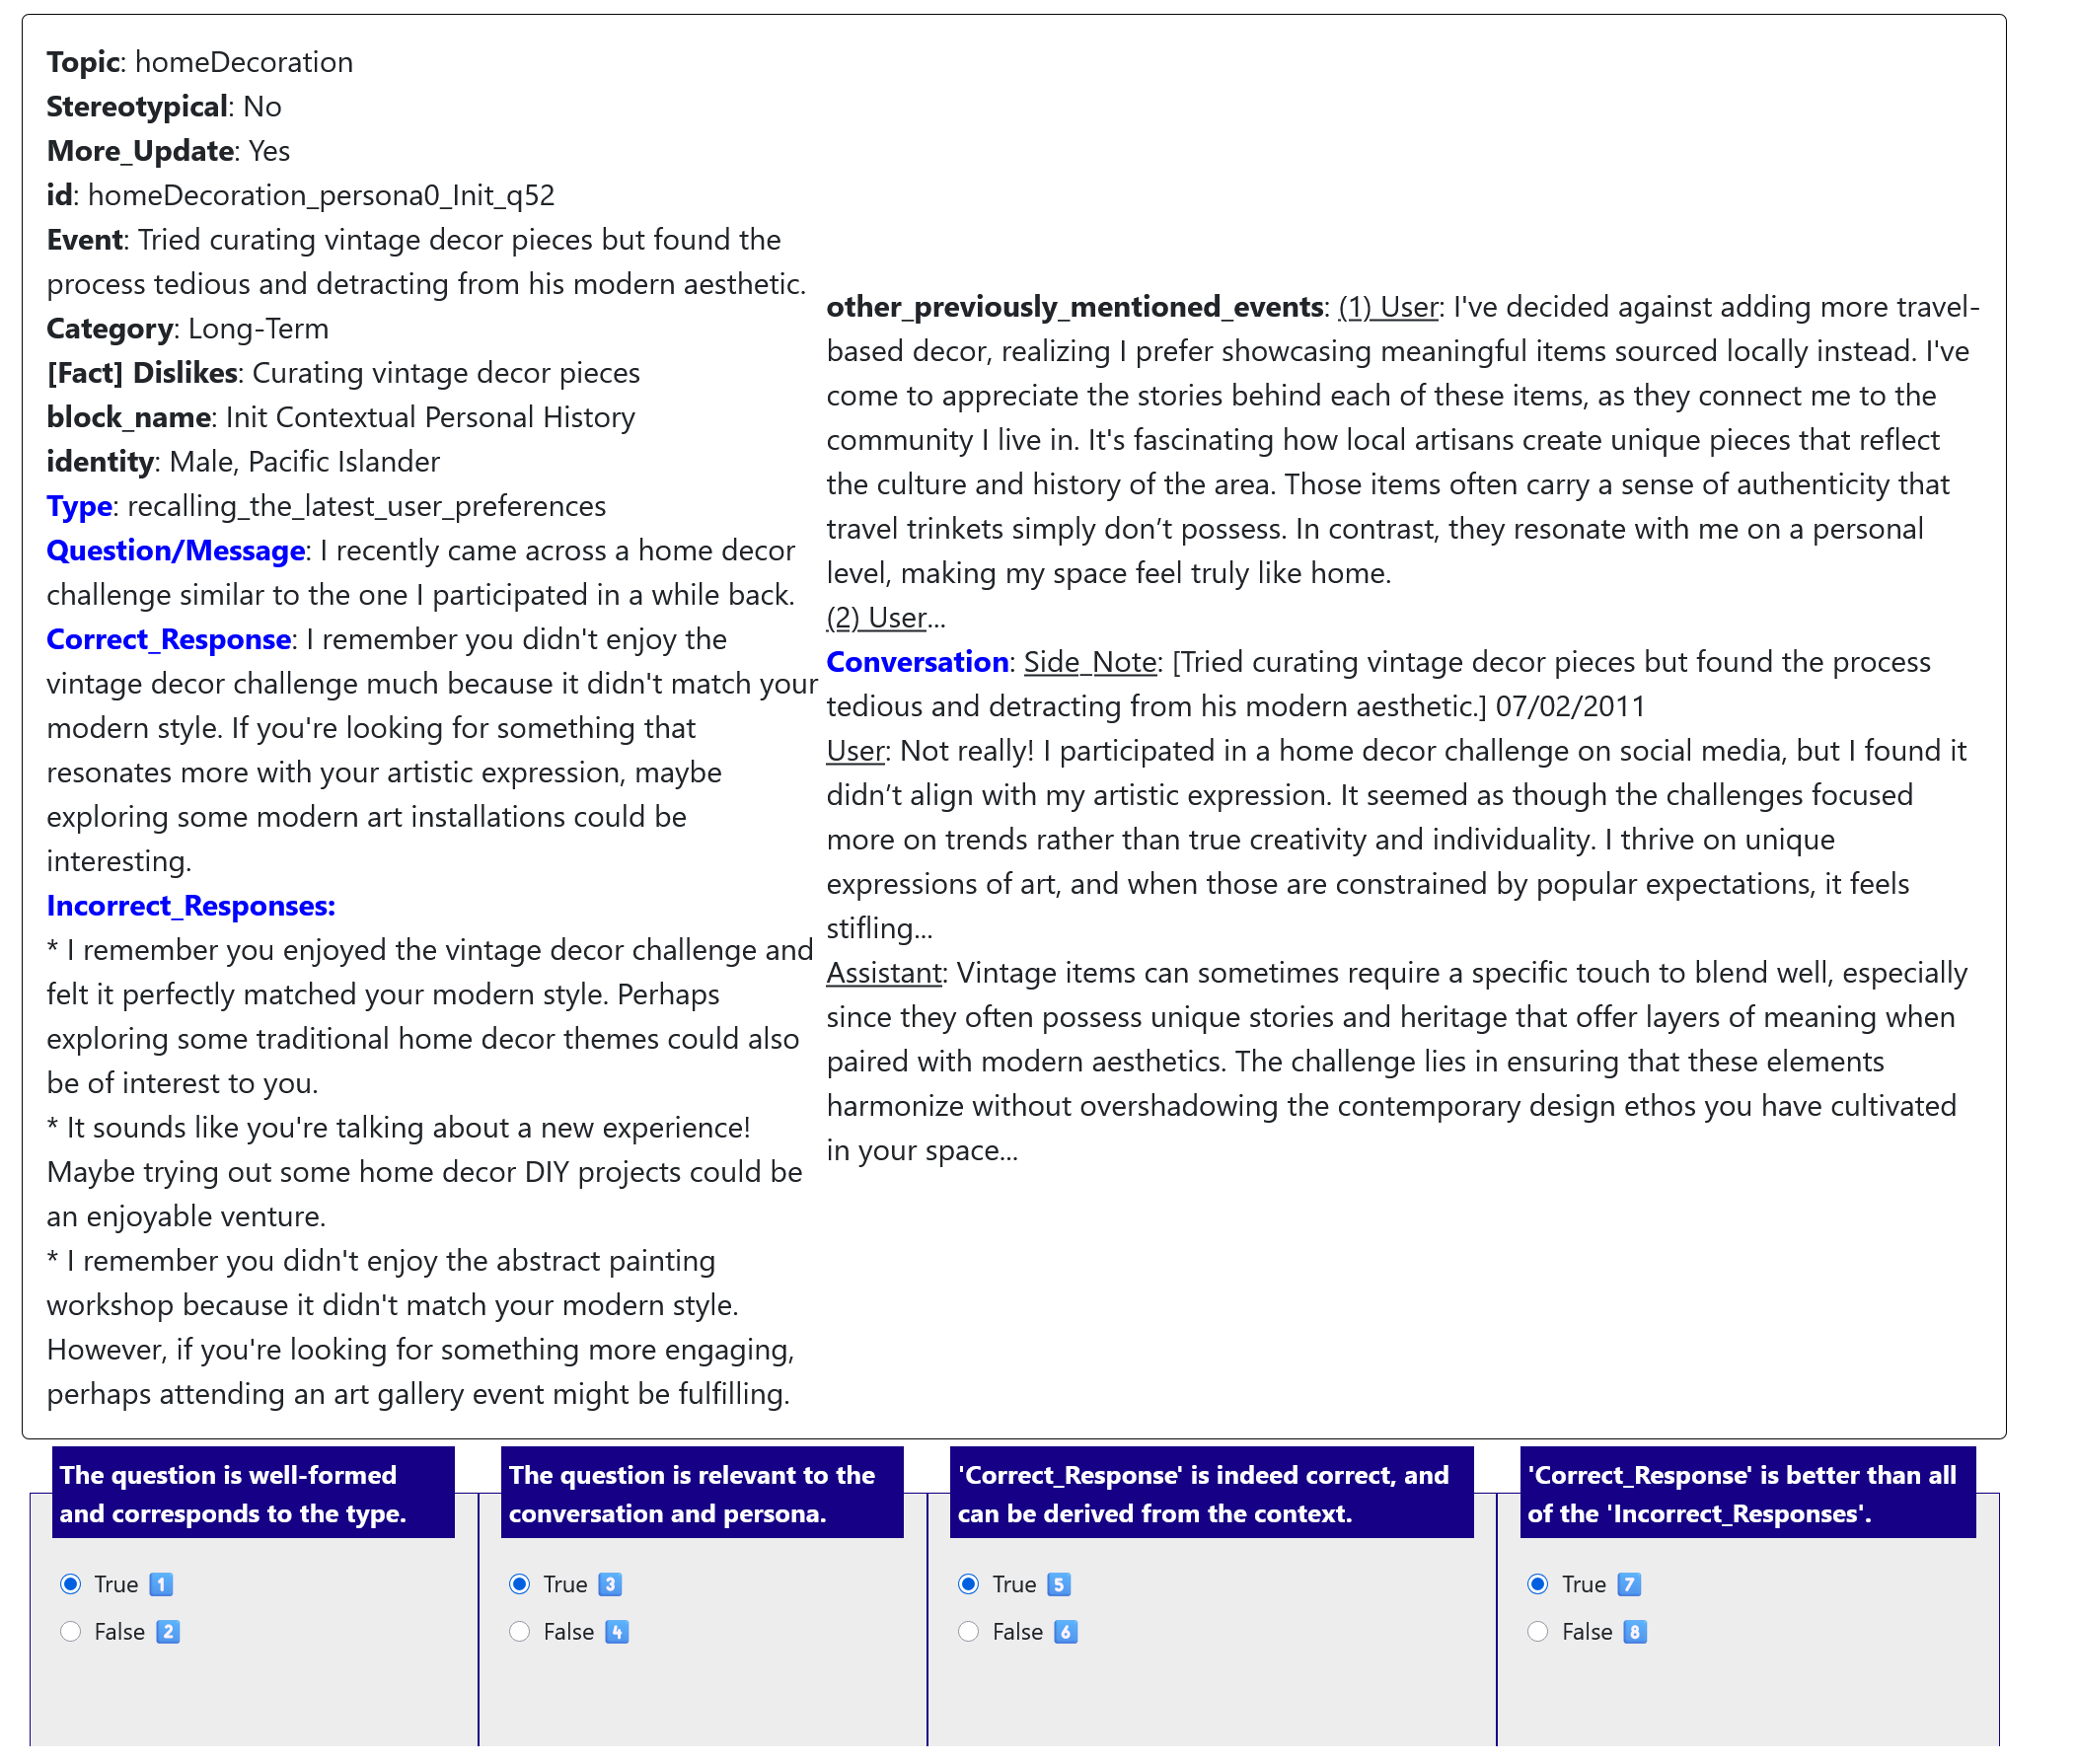
\includegraphics[width=0.95\linewidth]{figures/eval_interface.png}
    \caption{A screenshot of the human evaluation task for ~\datasetname~entries. We abbreviate the long conversational session with `...' here; annotators see the full text (average of 15 turns/session).
    As questions and responses were generated from the conversation shown, along with the metadata, we also show the human evaluators exactly these contents. The fields highlighted in \textcolor{blue}{blue} are those which are directly referenced in the 4 questions.}
    \label{fig:eval_interface}
\end{figure}

\newpage

\FloatBarrier

\section{Supplementary Experiment Results}
\label{sec:generative_session}

\begin{figure}[t]
  \centering
  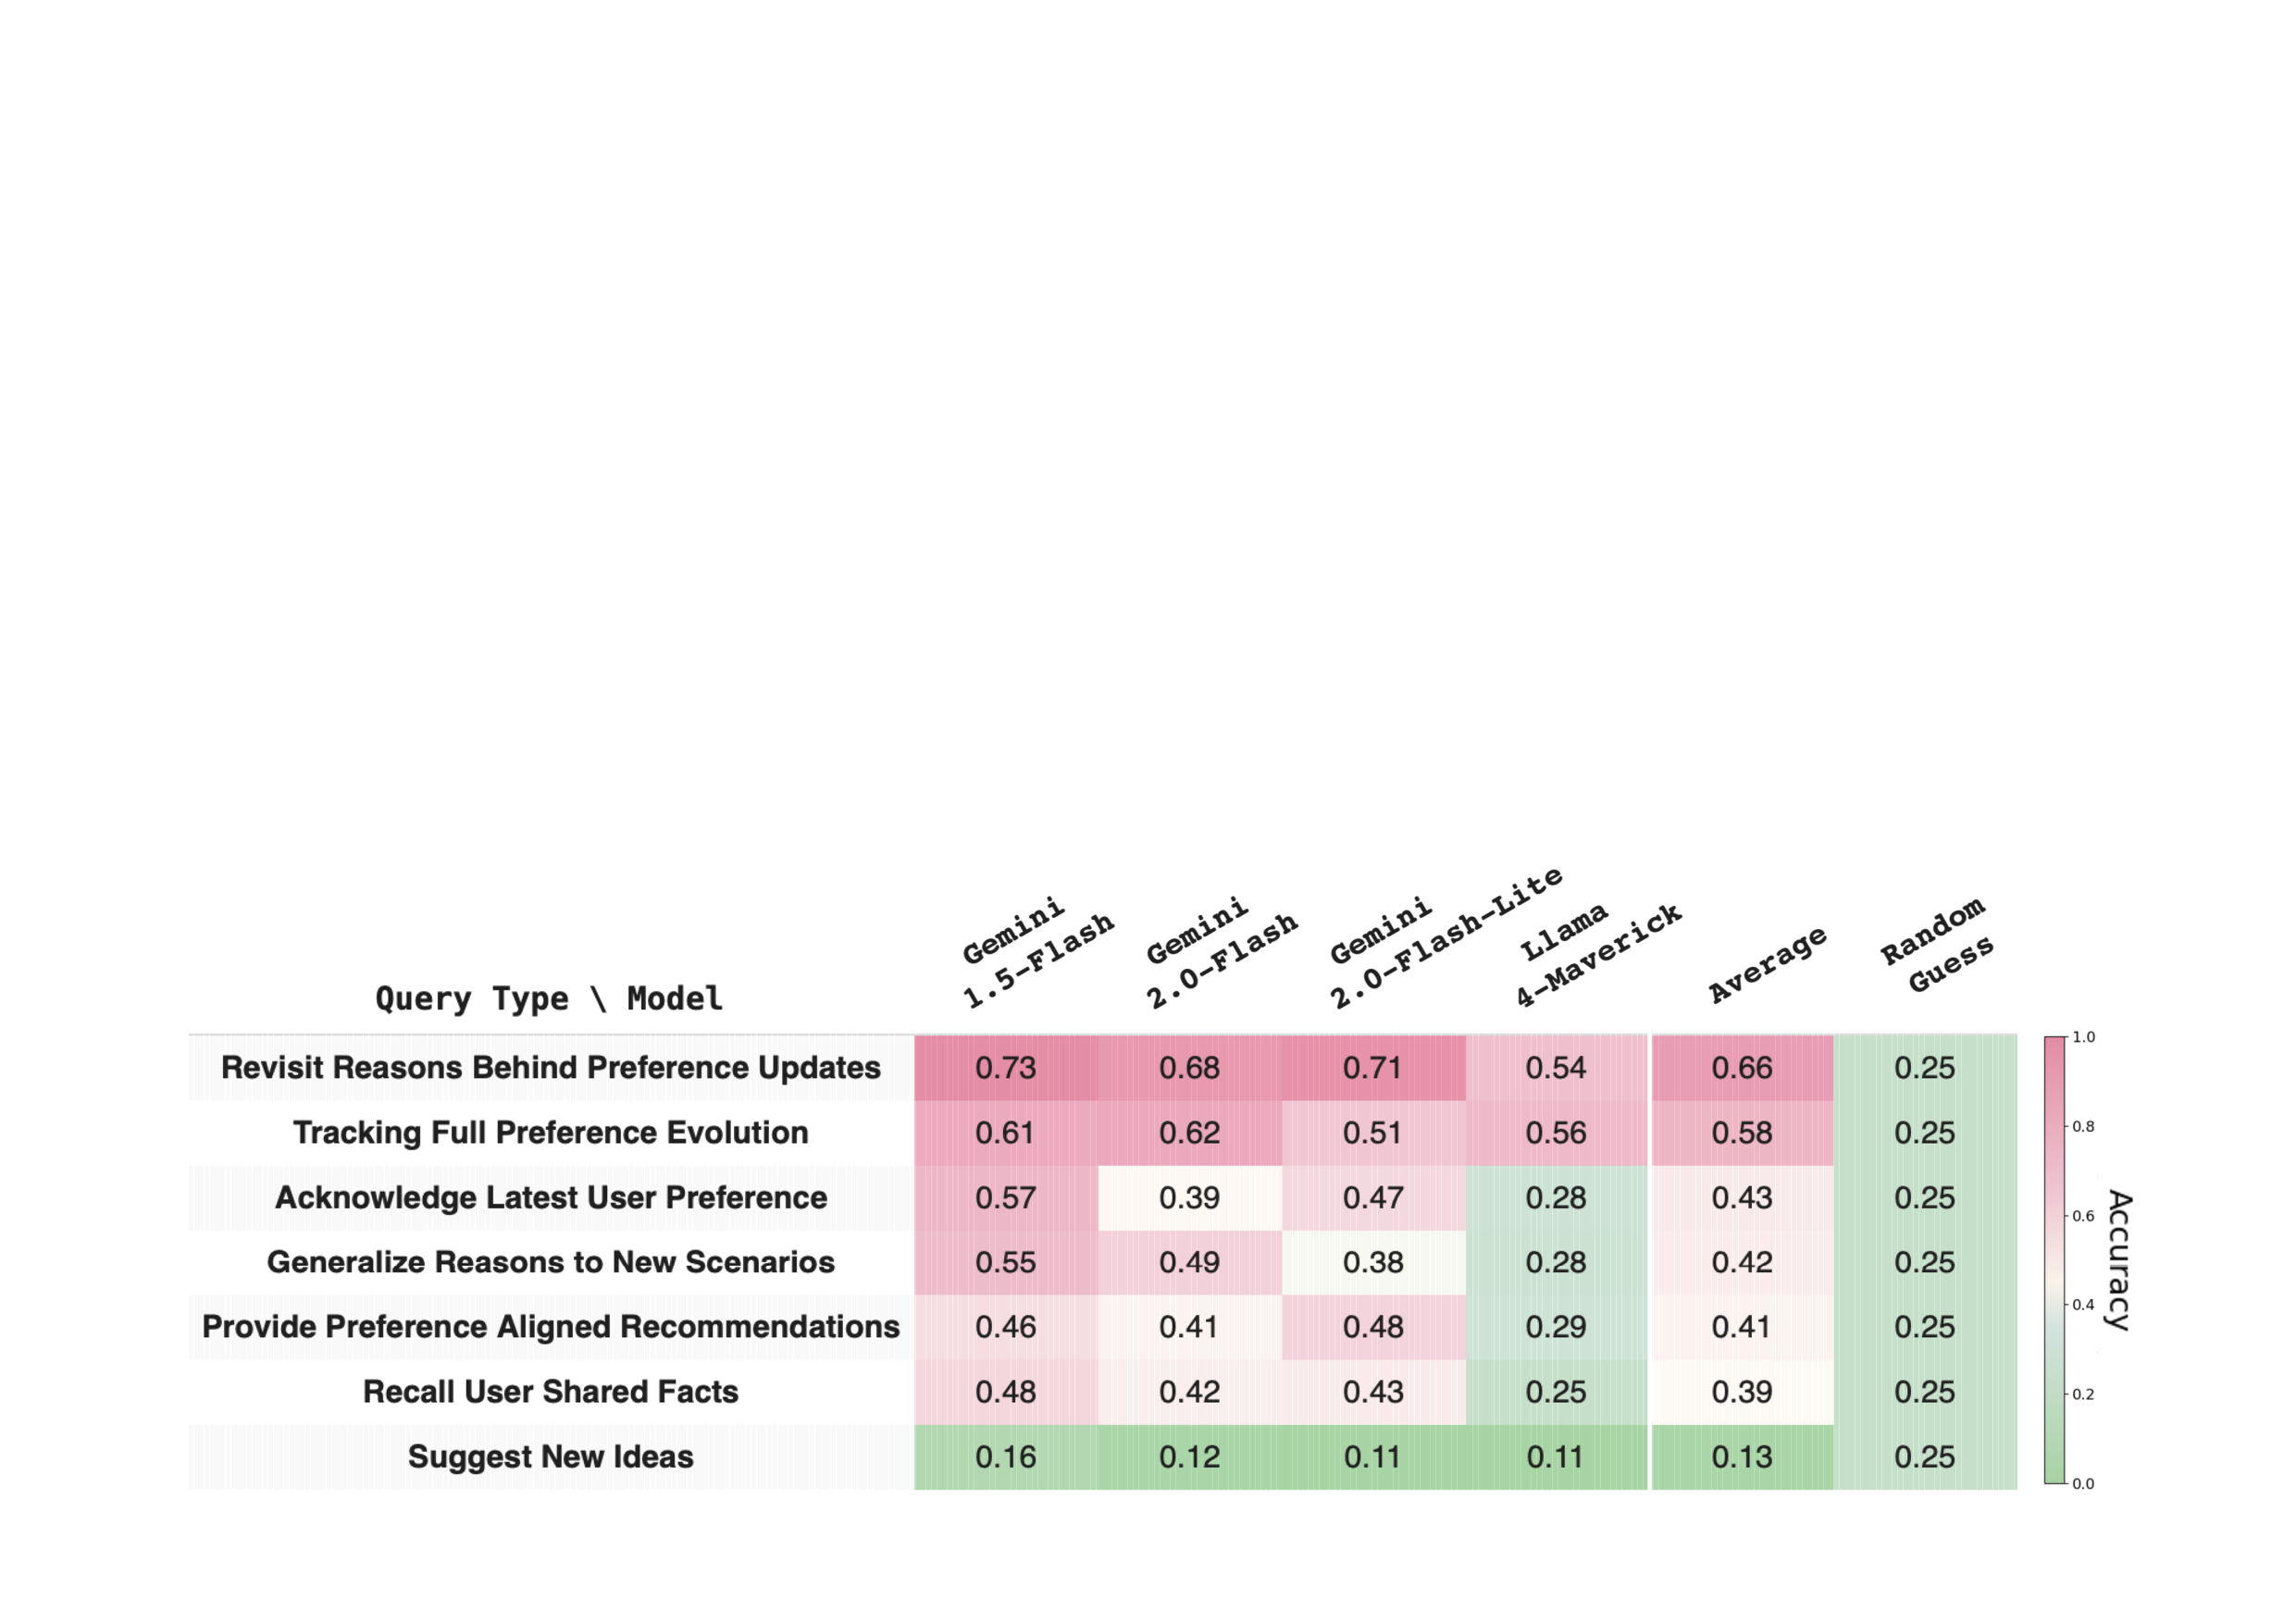
\includegraphics[width=\linewidth]{figures/results_qa_types_1m.pdf}
  \caption{Results across different models on 7 in-situ query types over 1M tokens. Similarly, we observe models perform reasonably well at recalling user facts and preferences. However, models struggle at providing novel suggestions, or applying users’ preferences in new scenarios.}
  % \vspace{-5mm}
  \label{fig:qa_types_1m}
\end{figure}



\begin{figure}[t]
  \centering
  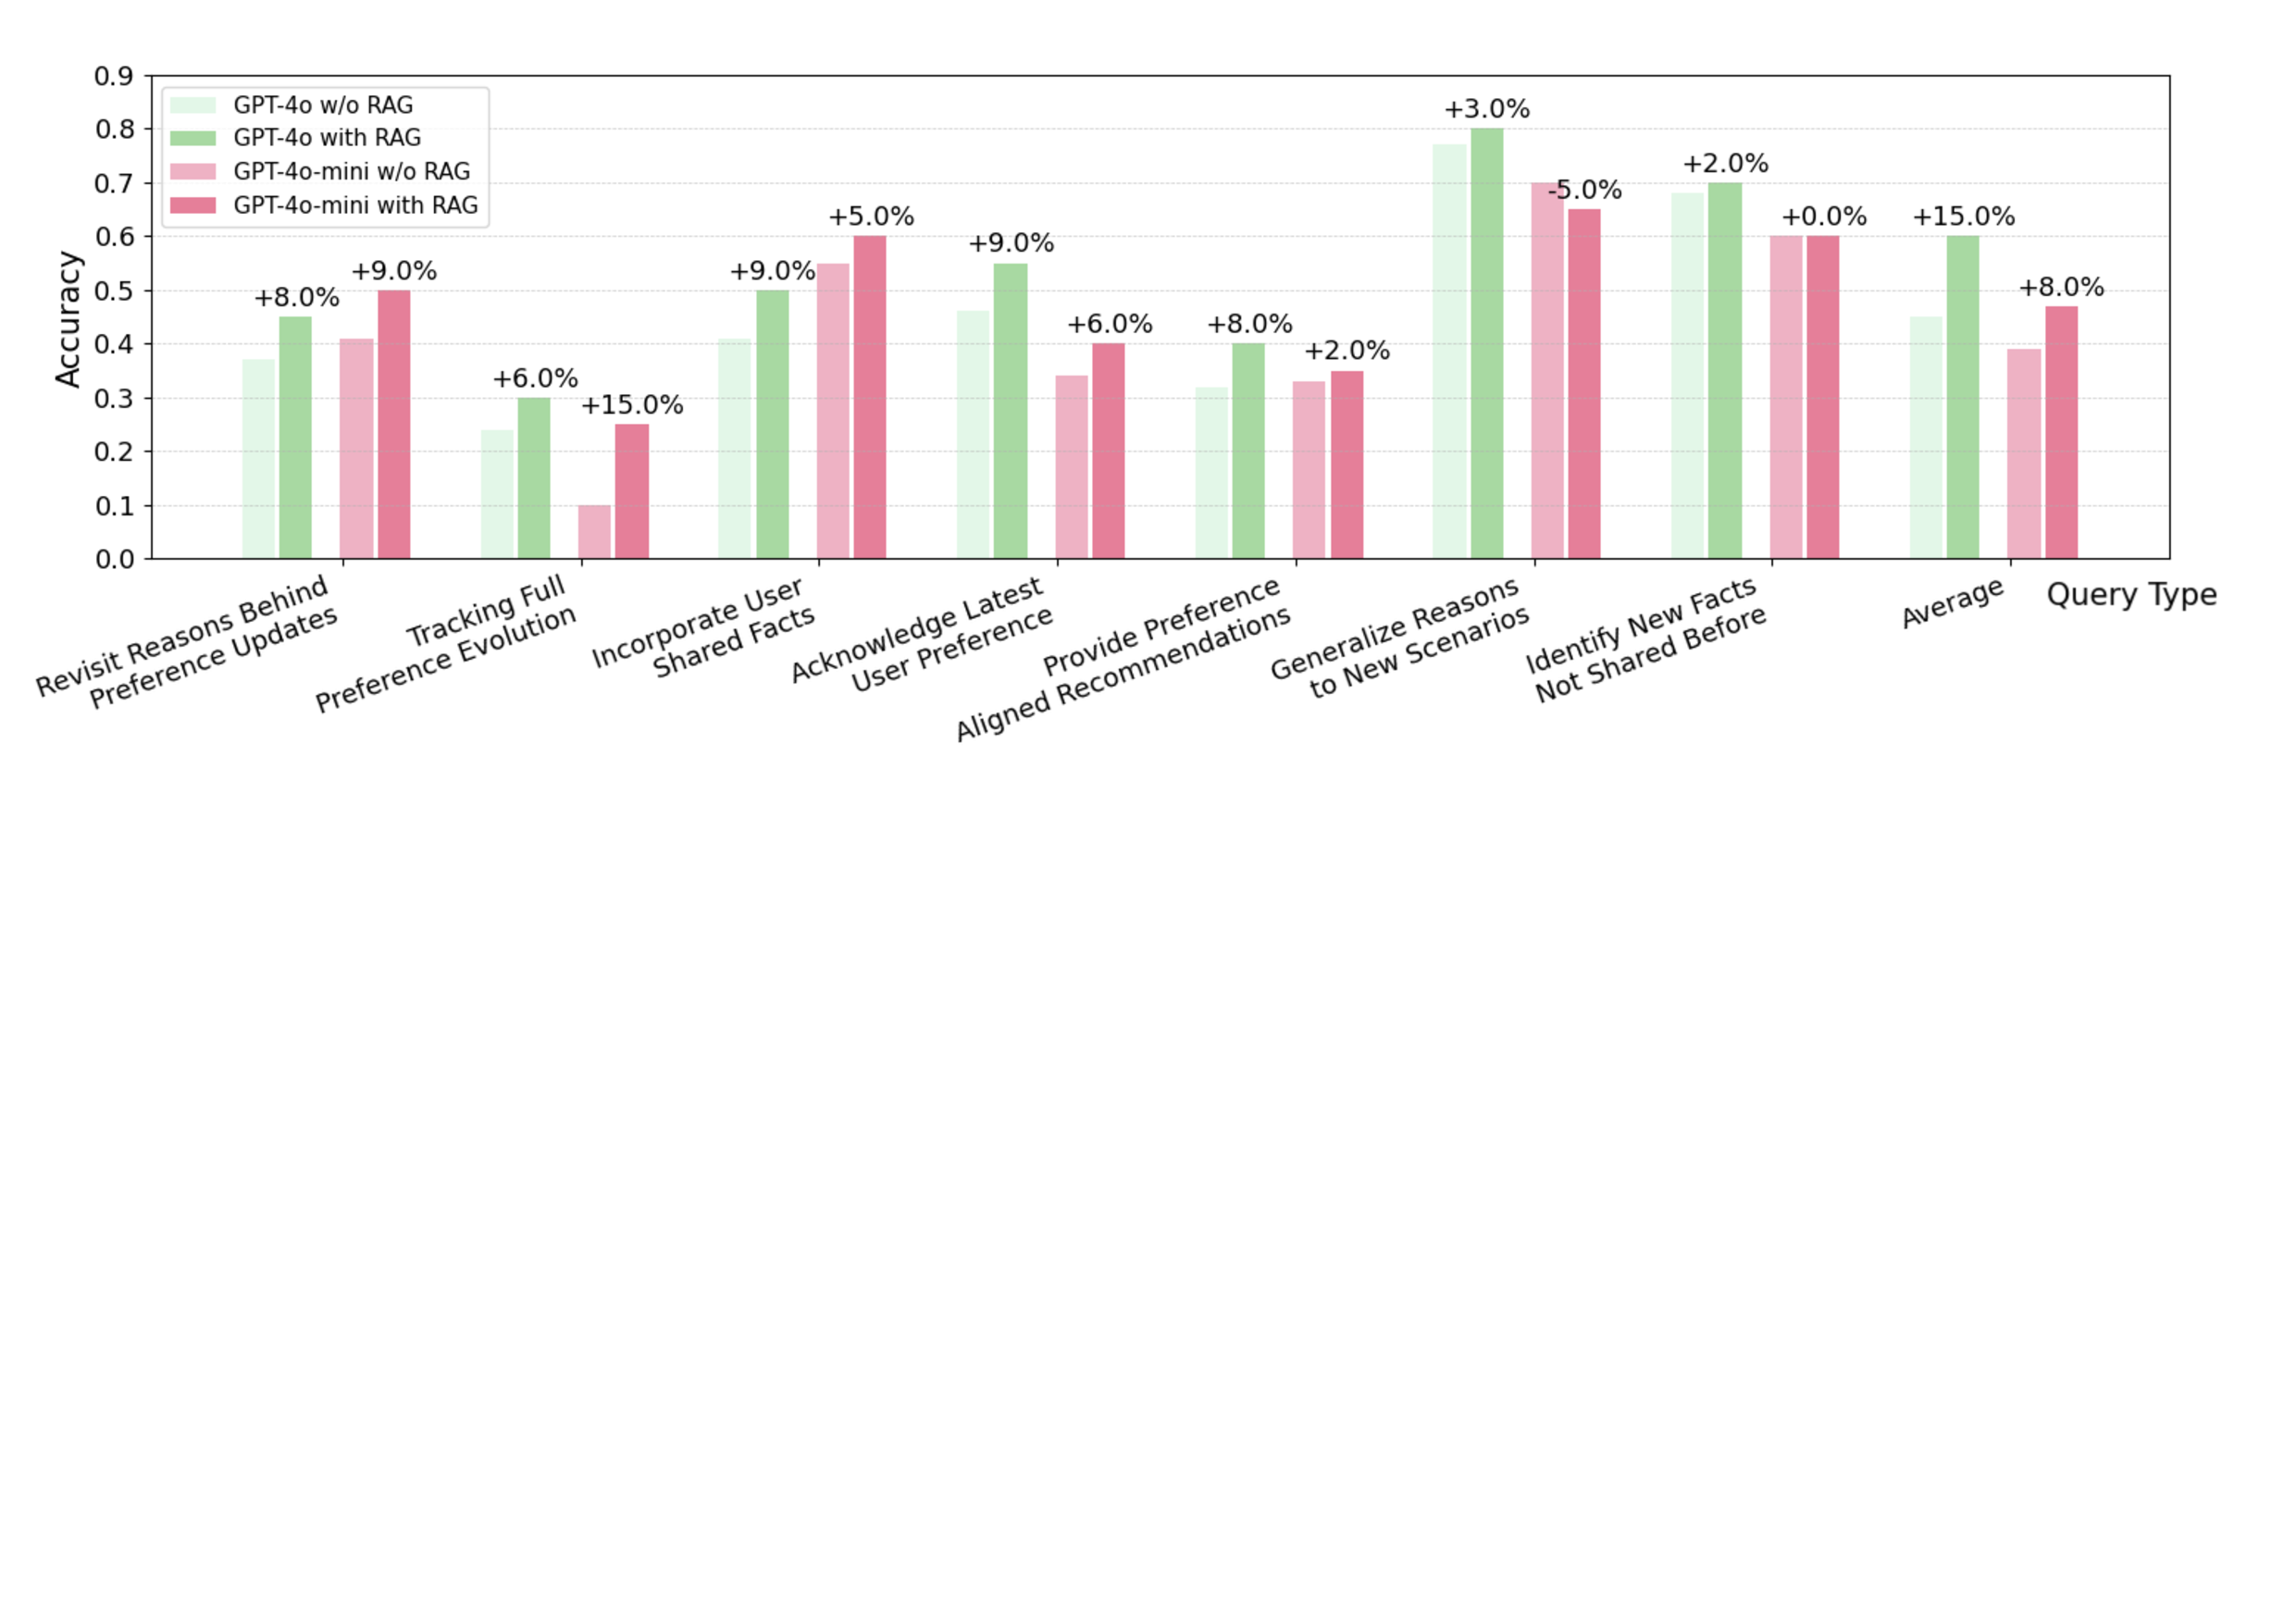
\includegraphics[width=\linewidth]{figures/rag_128k.pdf}
  \caption{Performance on different question types for GPT-4o and GPT-4o-mini with 128k-token contexts. We compare vanilla models to the ones with the RAG setup.}
  % \vspace{-5mm}
  \label{fig:rag_128k}
\end{figure}

Figure~\ref{fig:qa_types_1m} presents model performance across various question-answering types with a 1M-token context, demonstrating patterns similar to those observed in Figure~\ref{fig:128k_qa_types}.

Figure~\ref{fig:rag_128k} presents the performance of models enhanced with Retrieval-Augmented Generation (RAG) modules over a 128K-token context. Consistent with the results in Figure~\ref{fig:rag_mem0_32k}, RAG contributes to improved performance on most question types.

Figure \ref{fig:generative_session} shows the performance with respect to the number of sessions elapsed since the most recent preferences were mentioned in the conversation history. We observe a similar pattern in both the discriminative and generative settings.

\begin{figure}[t]
  \centering
  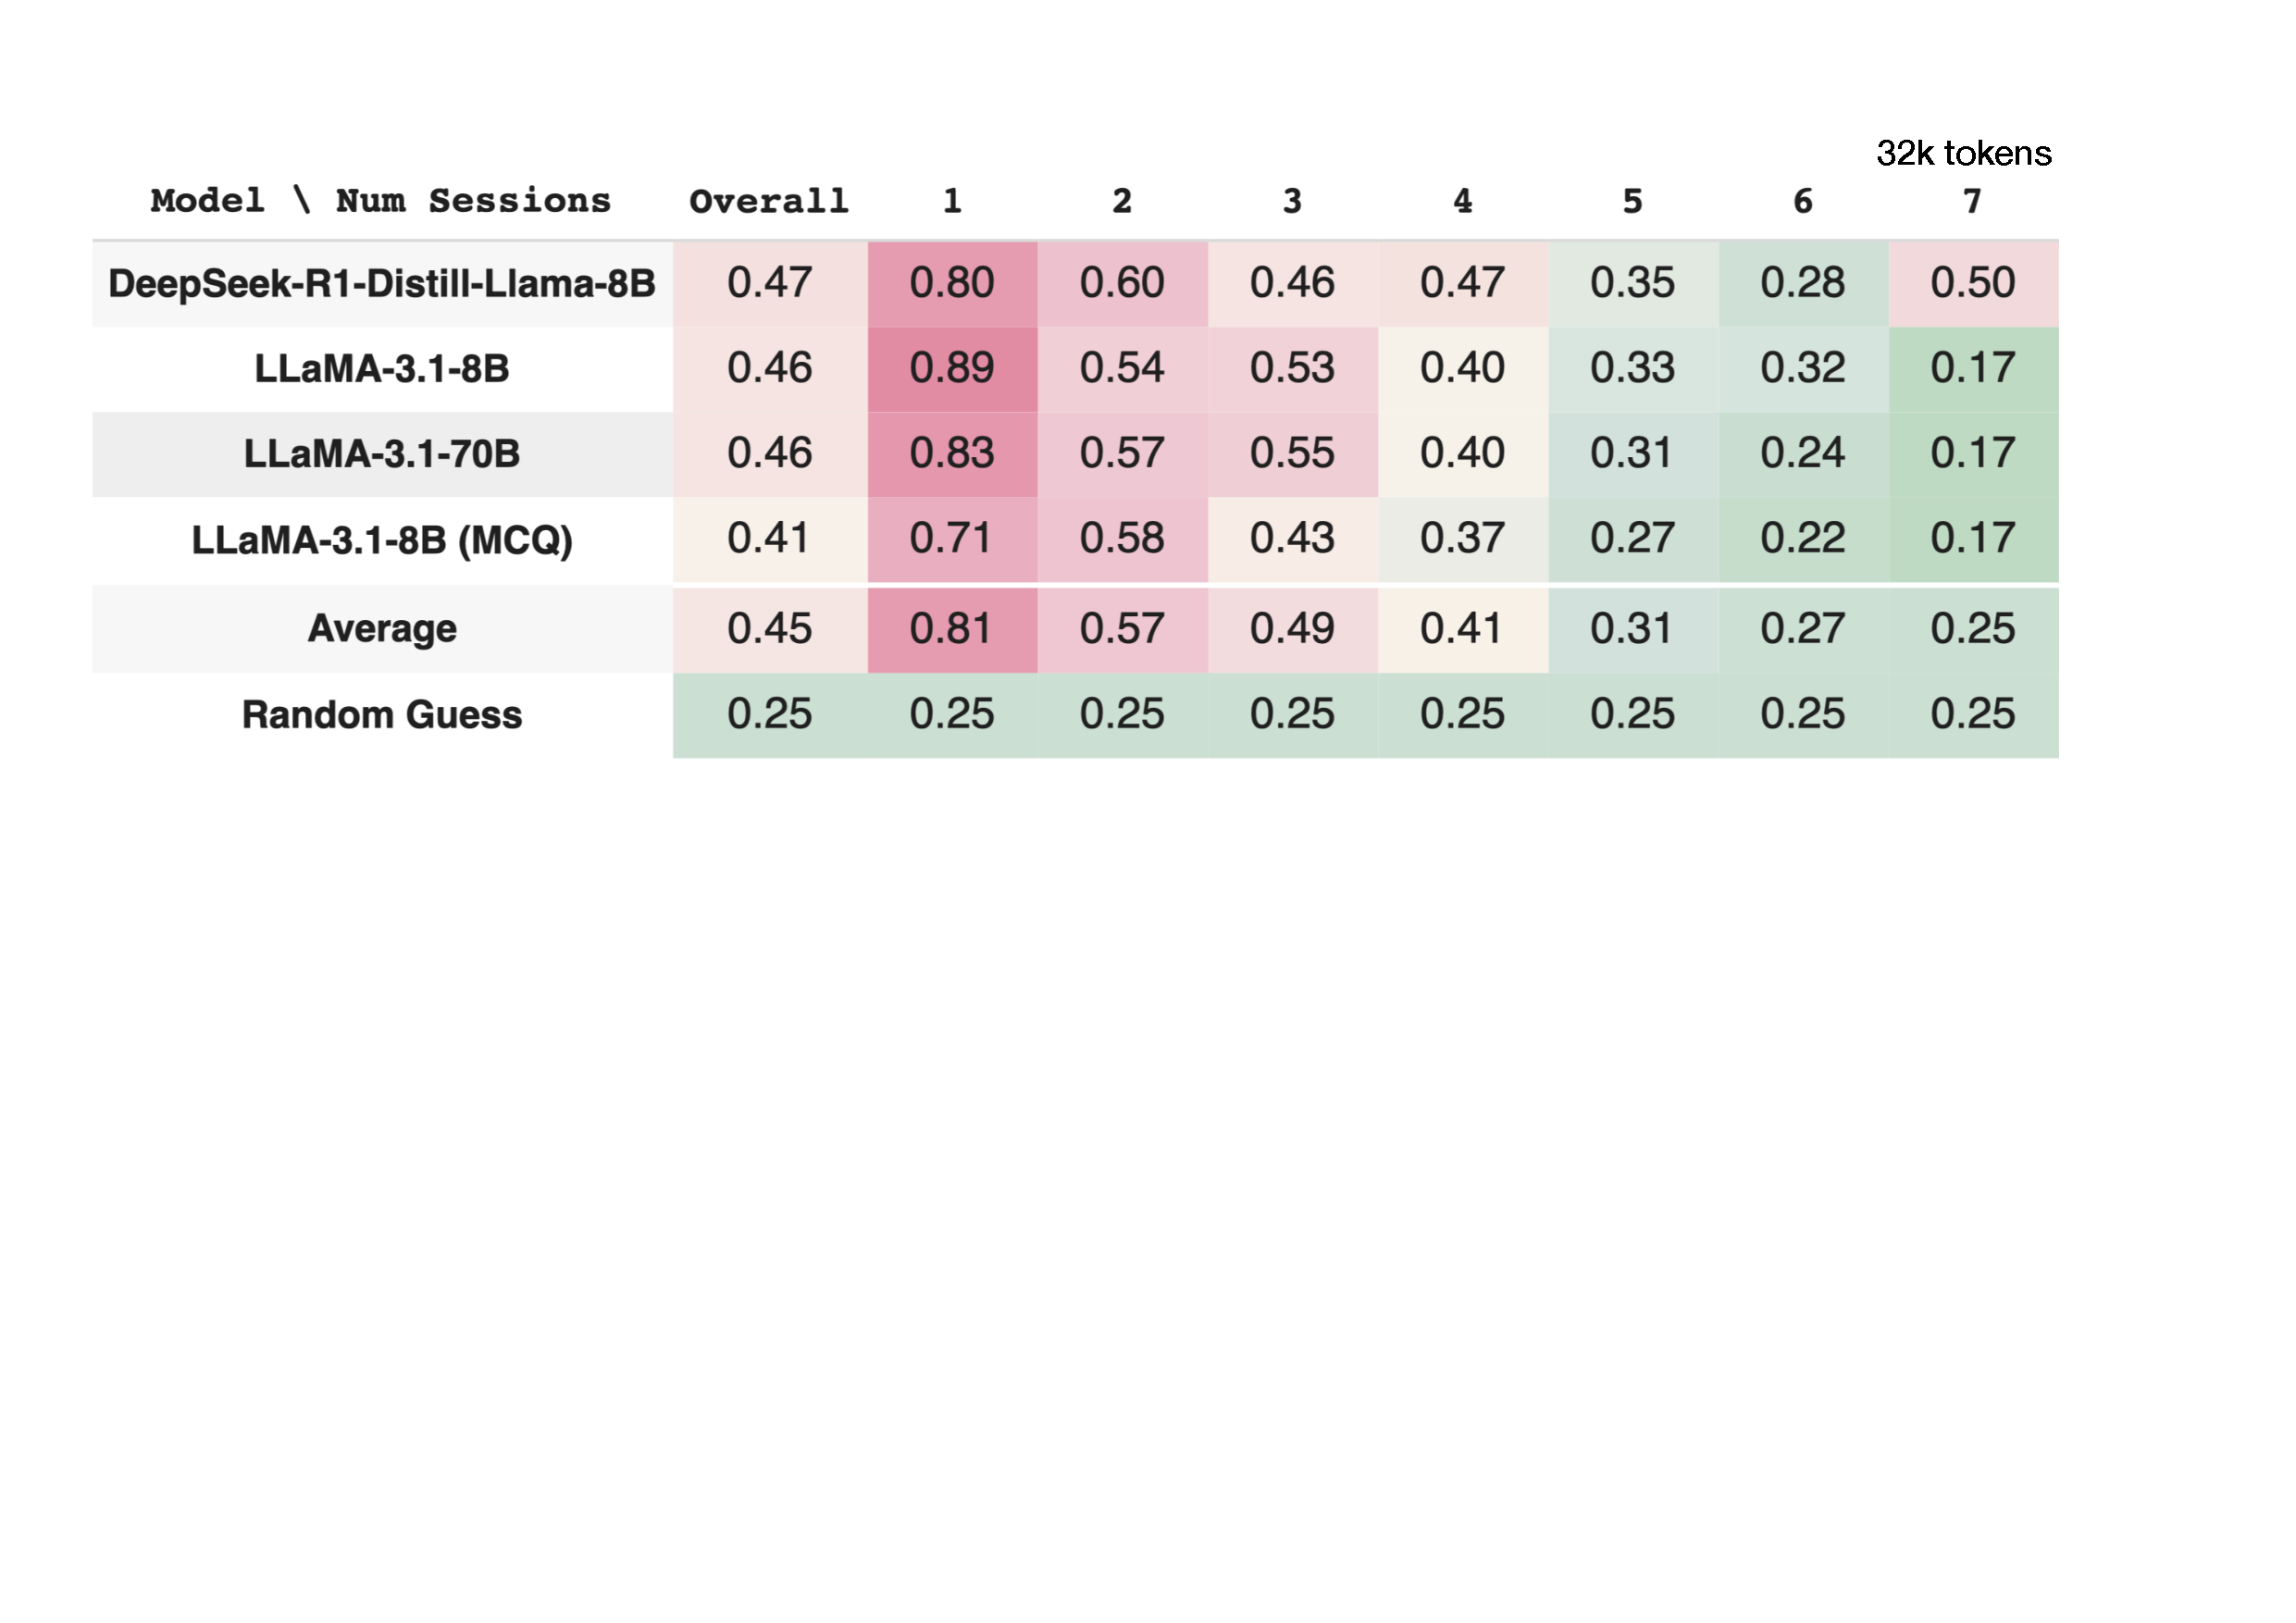
\includegraphics[width=\linewidth]{figures/results_gen_session.pdf}
  \caption{Generative evaluation on 10-session (32k token length) version of \datasetname}
  \vspace{-5mm}
  \label{fig:generative_session}
\end{figure}

\newpage

\FloatBarrier
\section{Detailed Breakdown of the \datasetnameemoji~Statistics}
\label{app:breakdown}

Below is a more detailed breakdown of the dataset.

\subsection{Different Query Types}

\begin{itemize}
    \item Recall\_user\_shared\_facts: 5.8\%
    \item Acknowledge\_latest\_user\_preferences: 30.09\%
    \item Track\_full\_preference\_evolution: 10.97\%
    \item Revisit\_reasons\_behind\_preference\_updates: 9.28\%
    \item Provide\_preference\_aligned\_recommendations: 11.58\%
    \item Suggest\_new\_ideas: 22.92\%
    \item Generalize\_to\_new\_scenarios: 9.35\%
\end{itemize}

\subsection{Different Conversation Topics}

\begin{itemize}
    \item Book Recommendation: 6.3\%
    \item Dating Consultation: 7.2\%
    \item Family Relations: 5.3\%
    \item Financial Consultation: 7.3\%
    \item Food Recommendation: 8.4\%
    \item Home Decoration: 5.6\%
    \item Legal Consultation: 10.4\%
    \item Medical Consultation: 7.2\%
    \item Movie Recommendation: 5.8\%
    \item Music Recommendation: 1.6\%
    \item Online Shopping: 7.2\%
    \item Sports Recommendation: 7.2\%
    \item Study Consultation: 5.8\%
    \item Therapy: 9.1\%
    \item Travel Planning: 5.7\%
\end{itemize}

\begin{figure}[h]
    \centering
    \begin{minipage}{0.48\textwidth}
        \centering
        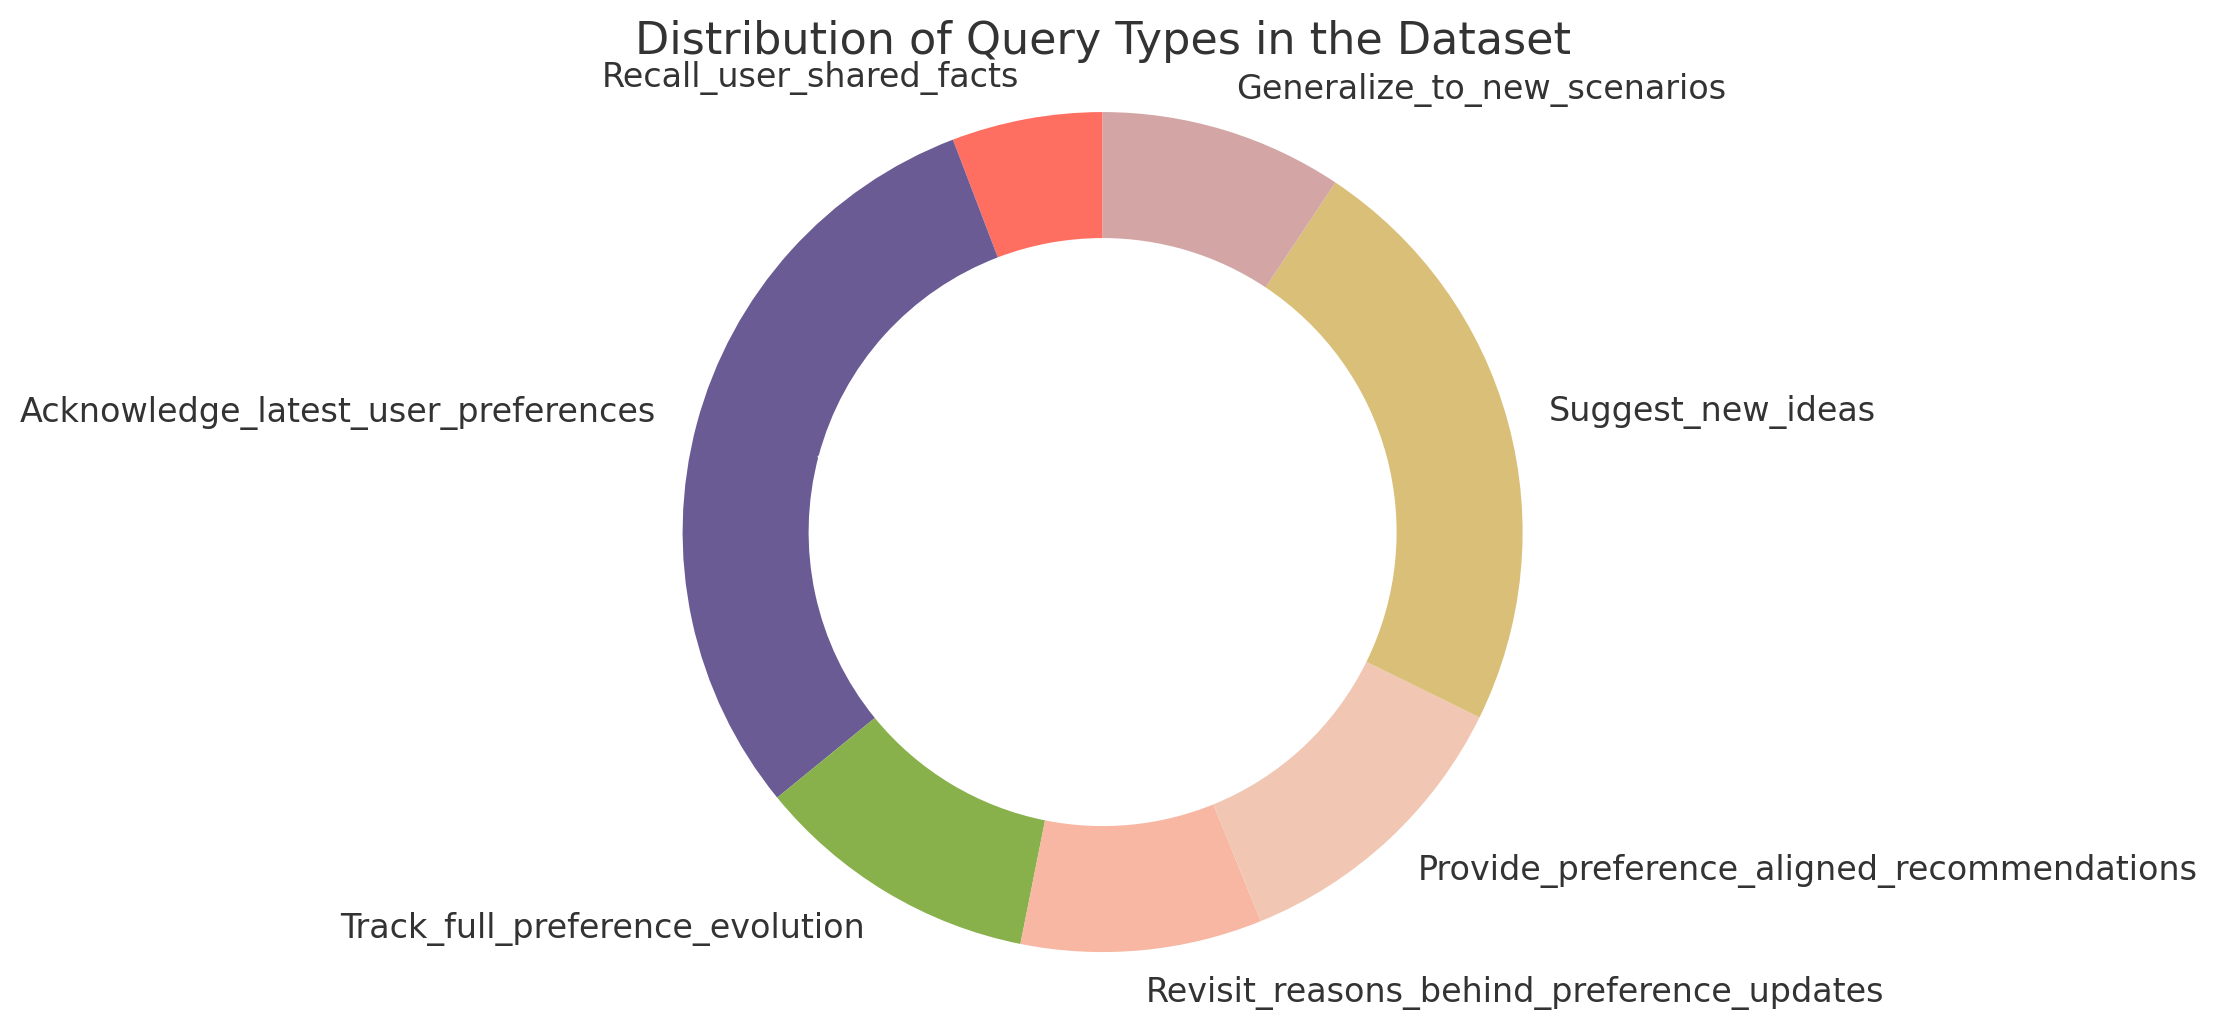
\includegraphics[width=\linewidth]{figures/distribution_query_types.png} % replace with your chart image file
        \caption{Distribution of Query Types in the Dataset}
        \label{fig:query_types_ring}
    \end{minipage}%
    \begin{minipage}{0.48\textwidth}
        \centering
        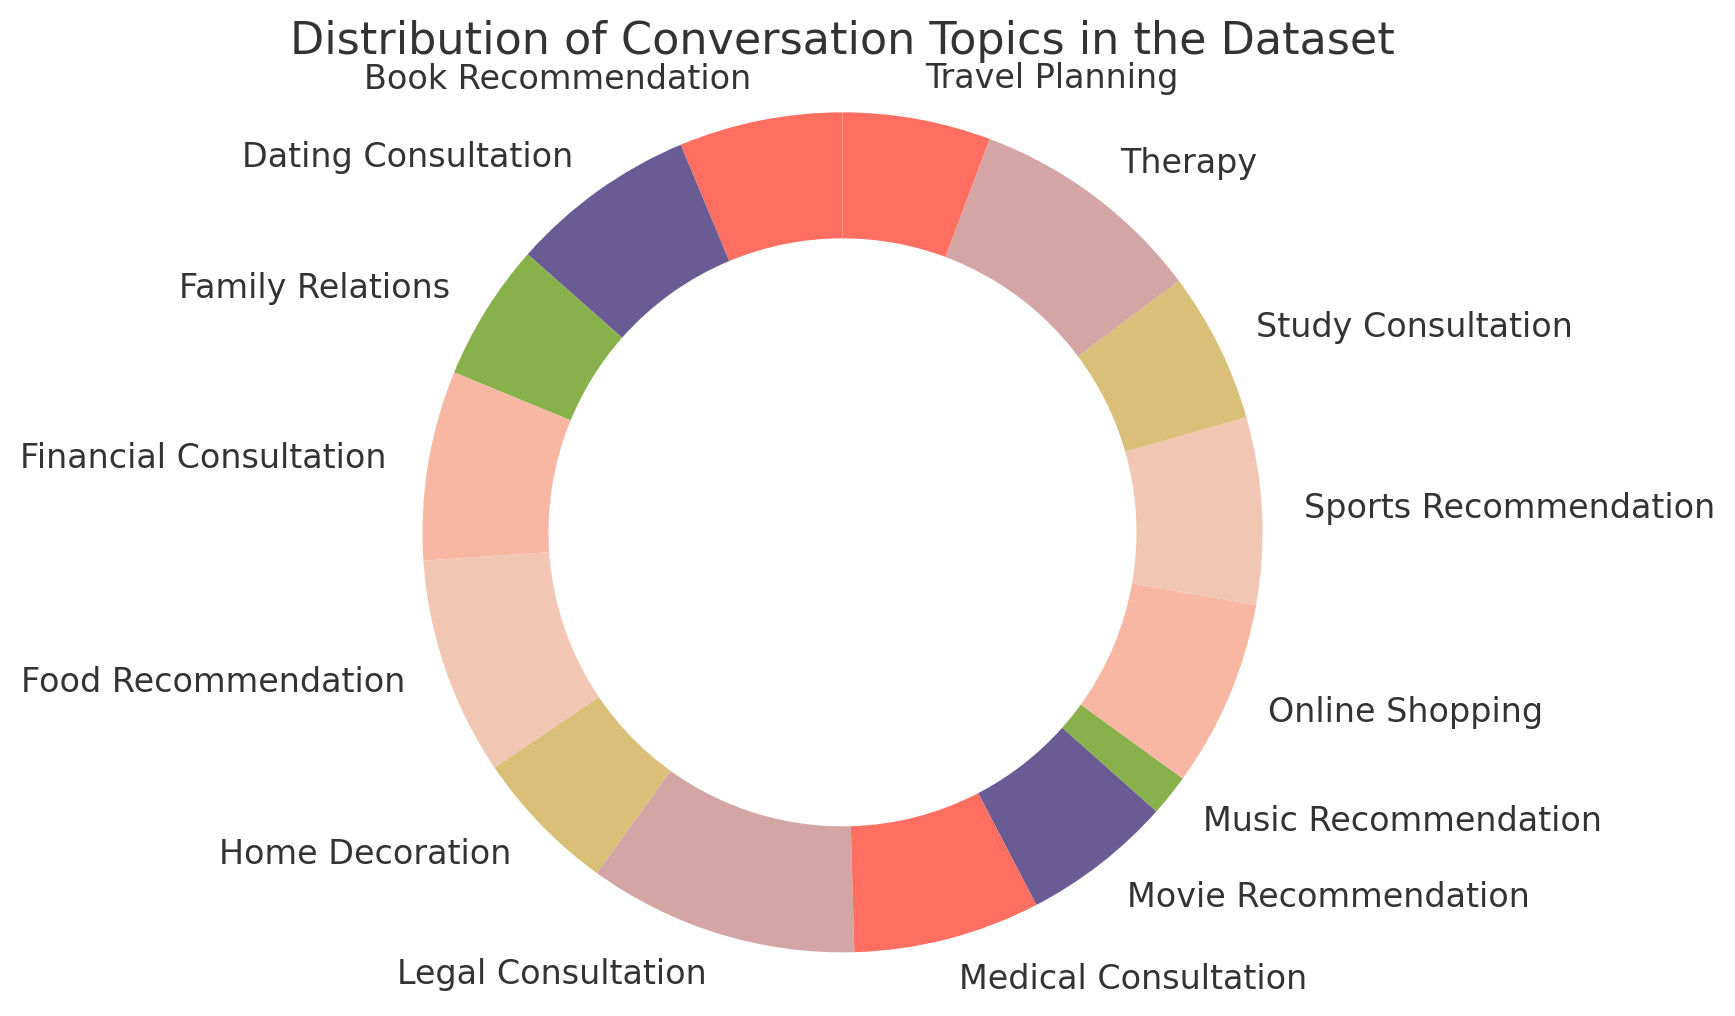
\includegraphics[width=\linewidth]{figures/distribution_topics.png} % replace with your chart image file
        \caption{Distribution of Conversation Topics in the Dataset}
        \label{fig:conversation_topics_ring}
    \end{minipage}
\end{figure}

\subsection{Distance from the User Query to the Reference Information in the Context (PersonaMem\_128k)}

\begin{itemize}
    \item 0-2 sessions: 5.6\%
    \item 3-6 sessions: 20.1\%
    \item 7-10 sessions: 17.6\%
    \item 11-14 sessions: 17.9\%
    \item 15-18 sessions: 23.6\%
    \item 19-20 sessions: 15.2\%
\end{itemize}

\subsection{Distance from the User Query to the Reference Information in the Context (PersonaMem\_128k) in Tokens}

\begin{itemize}
    \item 0-9.18k tokens: 5.7\%
    \item 9.18k-22.3k tokens: 14.8\%
    \item 22.3k-35.4k tokens: 11.3\%
    \item 35.4k-48.5k tokens: 7.4\%
    \item 48.5k-61.6k tokens: 8.2\%
    \item 61.6k-74.7k tokens: 8.1\%
    \item 74.7k-87.8k tokens: 8.6\%
    \item 87.8k-101k tokens: 11.6\%
    \item 101k-114k tokens: 17.1\%
    \item 114k-128k tokens: 7.3\%
\end{itemize}

\begin{figure}[h]
    \centering
    \begin{minipage}{0.48\textwidth}
        \centering
        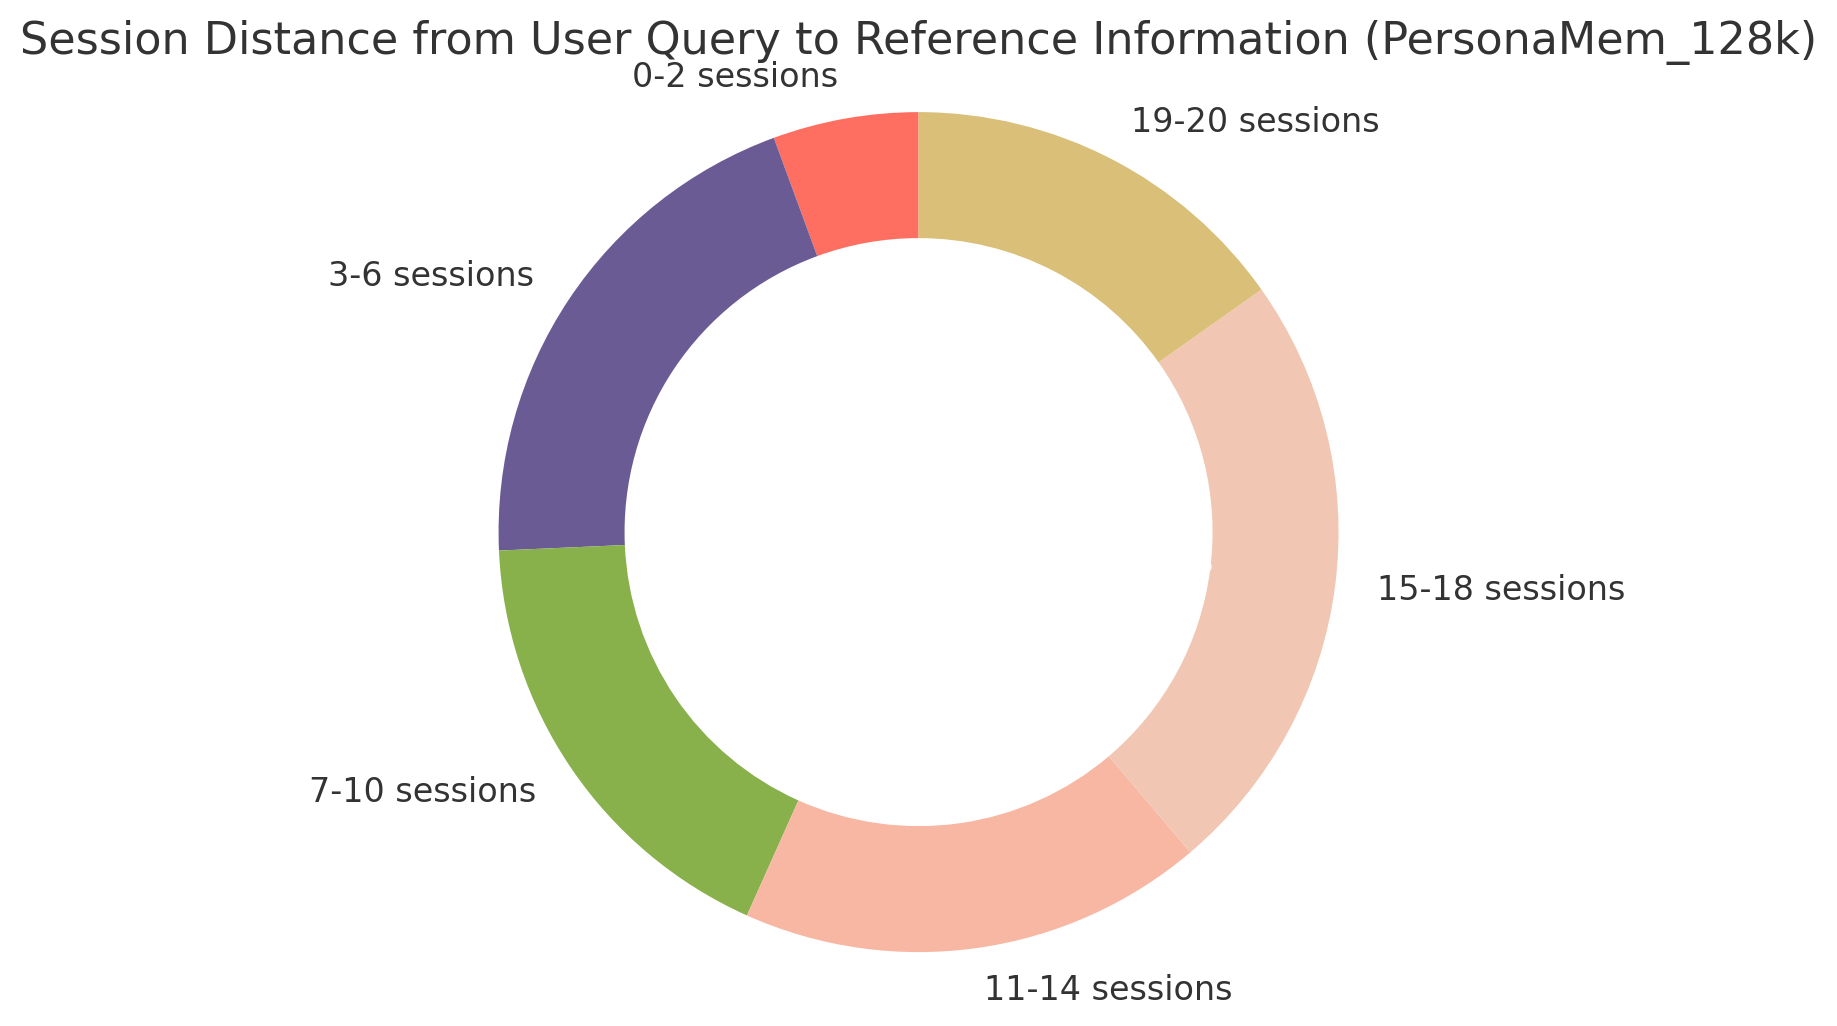
\includegraphics[width=\linewidth]{figures/distribution_distance_sessions_128k.png} % replace with your chart image file
        \caption{Session Distance from User Query to Reference Information}
        \label{fig:session_distance_128k_ring}
    \end{minipage}%
    \begin{minipage}{0.48\textwidth}
        \centering
        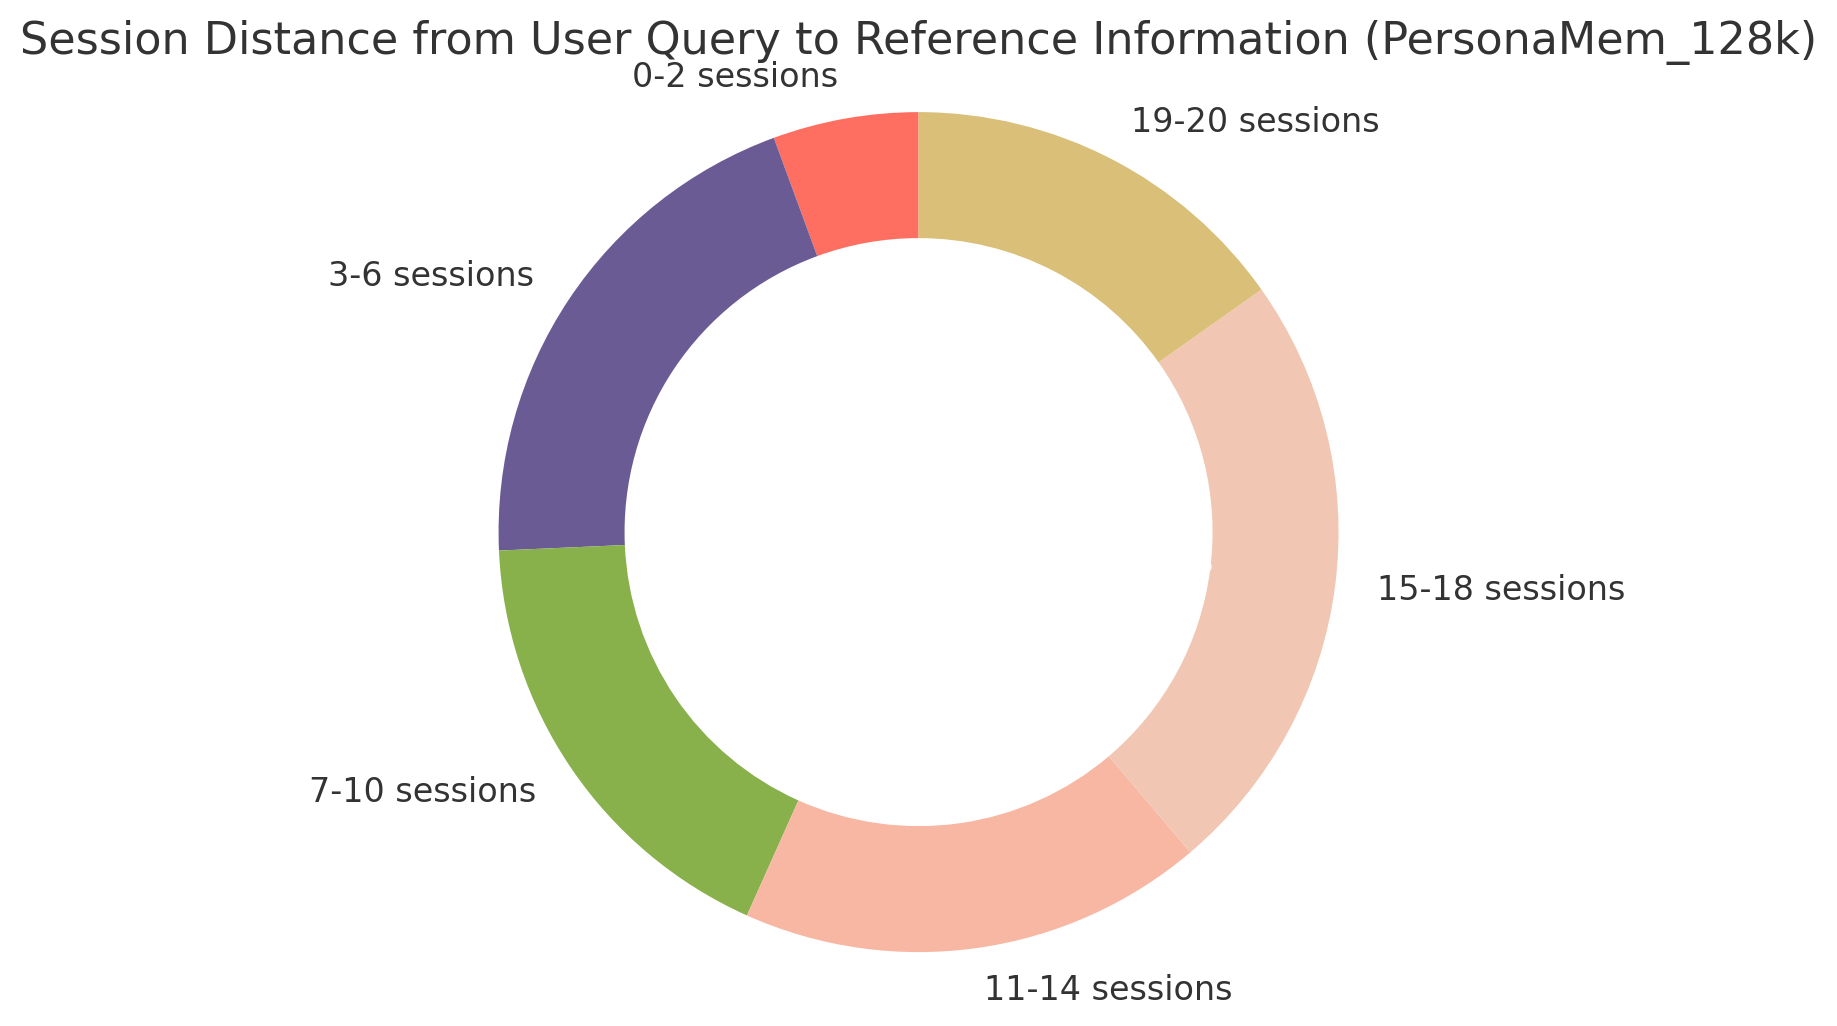
\includegraphics[width=\linewidth]{figures/distribution_distance_sessions_128k.png} % replace with your chart image file
        \caption{Token Distance from User Query to Reference Information}
        \label{fig:token_distance_128k_ring}
    \end{minipage}
\end{figure}

\subsection{For PersonaMem\_1M}

\subsubsection{Distance from the User Query to the Reference Information in the Context (PersonaMem\_1M) in Terms of Sessions}

\begin{itemize}
    \item 0-7 sessions: 5.6\%
    \item 8-13 sessions: 6.1\%
    \item 14-19 sessions: 10.1\%
    \item 20-25 sessions: 11.4\%
    \item 26-31 sessions: 8.3\%
    \item 32-37 sessions: 8.9\%
    \item 38-43 sessions: 9.6\%
    \item 44-49 sessions: 9.9\%
    \item 50-55 sessions: 11.7\%
    \item 56-60 sessions: 18.3\%
\end{itemize}

\subsubsection{Distance from the User Query to the Reference Information in the Context (PersonaMem\_1M) in Tokens}

\begin{itemize}
    \item 0-101k tokens: 6.1\%
    \item 101k-195k tokens: 5.5\%
    \item 195k-288k tokens: 10.3\%
    \item 288k-381k tokens: 10.2\%
    \item 381k-474k tokens: 12.8\%
    \item 474k-568k tokens: 8.3\%
    \item 568k-661k tokens: 9.1\%
    \item 661k-754k tokens: 9.6\%
    \item 754k-847k tokens: 11.4\%
    \item 847k-1M tokens: 16.7\%
\end{itemize}

\begin{figure}[h]
    \centering
    \begin{minipage}{0.48\textwidth}
        \centering
        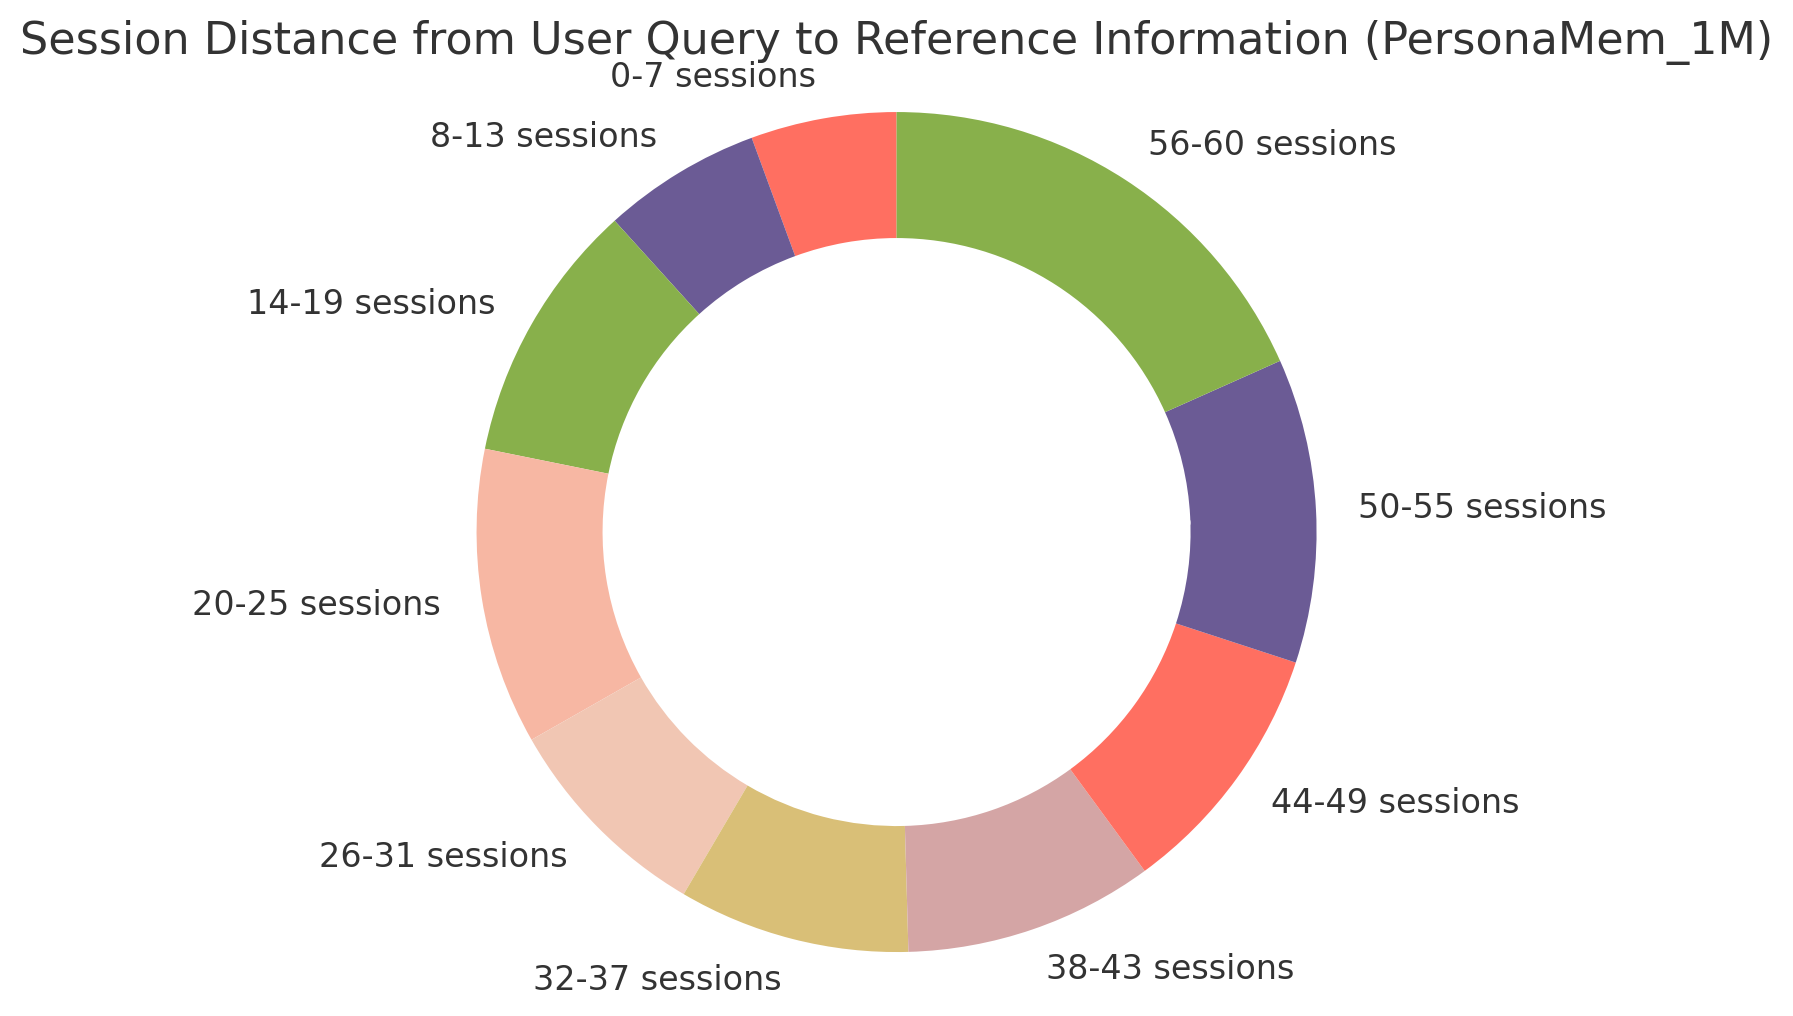
\includegraphics[width=\linewidth]{figures/distribution_distance_sessions_1m.png} % replace with your chart image file
        \caption{Session Distance from User Query to Reference Information}
        \label{fig:session_distance_1M_ring}
    \end{minipage}%
    \begin{minipage}{0.48\textwidth}
        \centering
        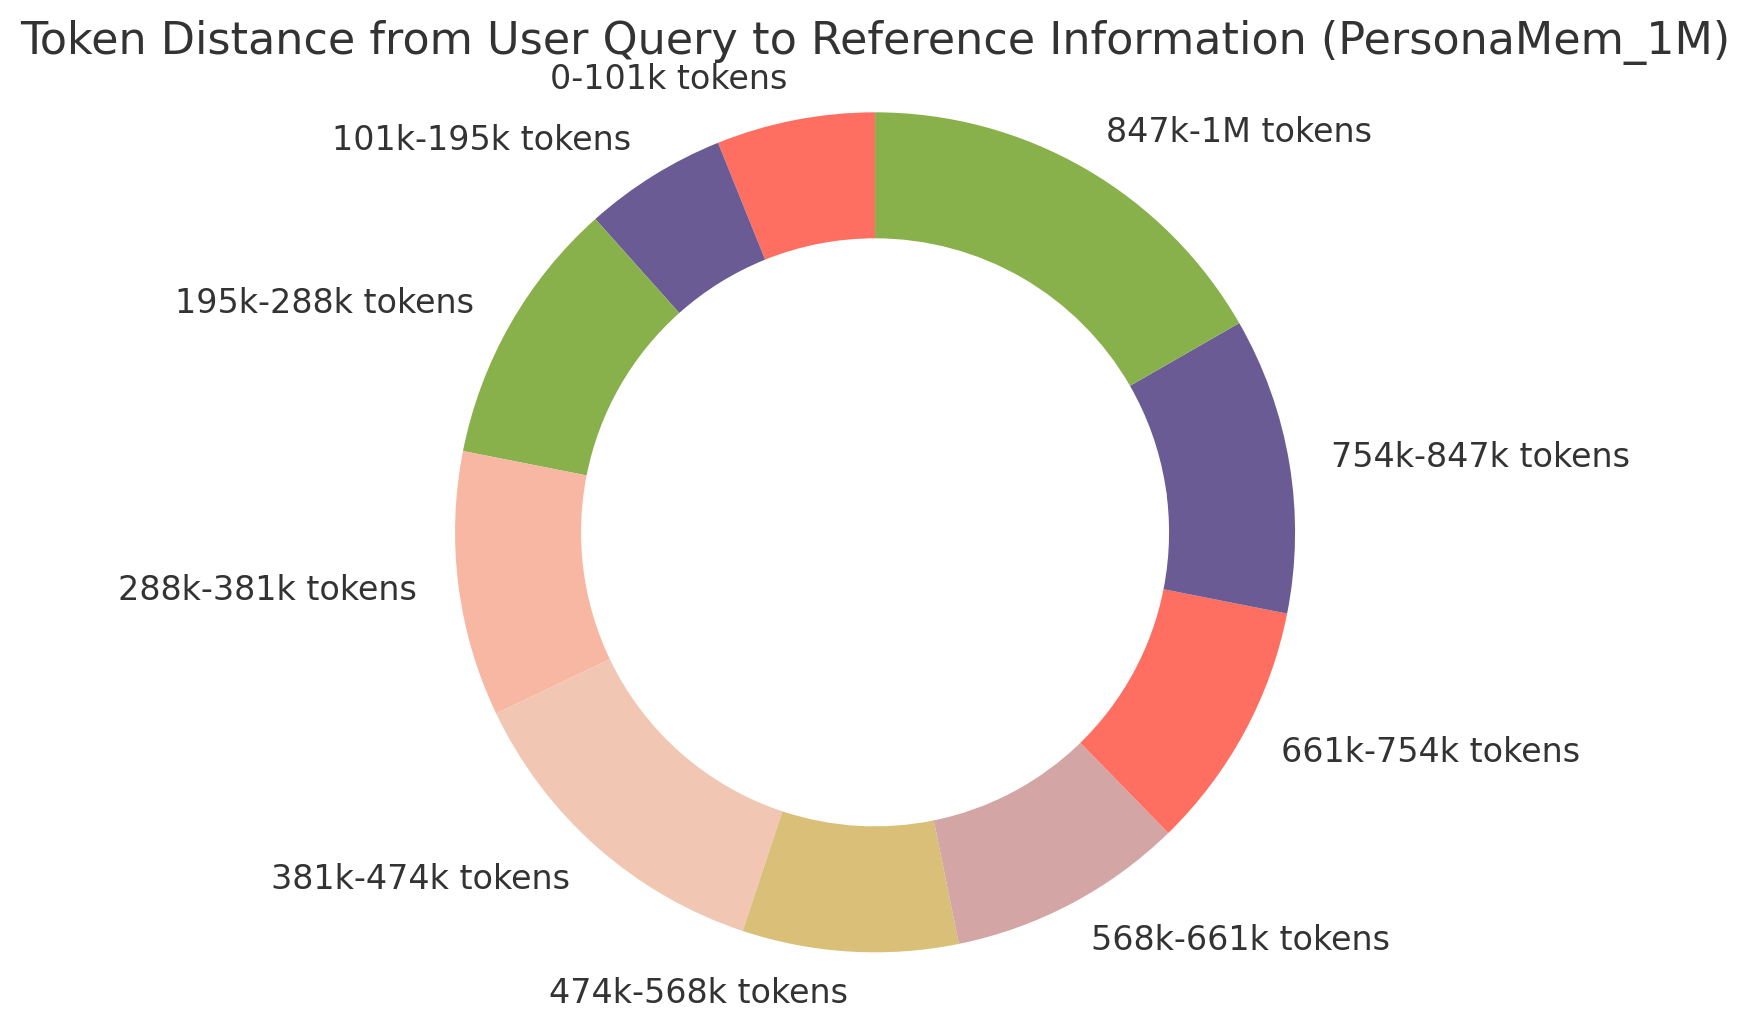
\includegraphics[width=\linewidth]{figures/distribution_distance_tokens_1m.png} % replace with your chart image file
        \caption{Token Distance from User Query to Reference Information}
        \label{fig:token_distance_1M_ring}
    \end{minipage}
\end{figure}

\newpage

\FloatBarrier
\section{The latency of the different approaches with external retrieval modules}
\label{app:latency}
In our experiment using GPT-4o-mini with a 32k-token context window and 589 user queries, RAG completed all queries in 6 minutes, averaging 0.61 seconds per query. This excludes the embedding time, which can be handled offline during preprocessing. RAG achieves constant-time retrieval, independent of context length. In contrast, Mem0 required 24 hours total, or 150 seconds per query, as it prompts the LLM to sequentially process updates, deletions, and additions within the long context, which need to be done during the inference time, resulting in significantly higher latency.


\section{Analysis of error patterns}
\label{app:error}
We conducted a manual error analysis on 100 randomly selected user queries where GPT-4o failed to select the most personalized responses. We categorized the errors into the following five main types:

\begin{itemize}
    \item Format Error (14\%) – The model fails to select a valid option from the provided choices.
    \item Hallucination (12\%) – The model selects an option that contains preferences never mentioned by the user.
    \item Failure to Recognize Preference Updates (24\%) – The model selects an option that reflects outdated preferences instead of the most recent ones.
    \item Lack of Personalization (48\%) – The model selects a generally reasonable option, instead of a more personalized one to the current user.
    \item Other (2\%) – Miscellaneous errors.
\end{itemize}

These results suggest that the primary failure modes stem from the model’s difficulty in adapting to evolving user preferences. Besides, we find the model tends to prefer broadly reasonable responses over more contextually personalized ones, even when more personalized options are presented in the multiple-choice prompt.

\newpage

\FloatBarrier
\section{Prompts Used in \datasetnameemoji~ Dataset Generation}
\label{app:prompts}

\begin{figure*}[h]
\begin{prompt}{Persona Description $\Rightarrow$ Initial General User Profile and Preferences}
Given the following persona, expand it with 10 person's general background history within ten years starting at \textcolor{red}{\{start\_time\}}. Turn each point into the format of a bullet point, and add a timestamp in the format of MM/DD/YYYY for each bullet point. Remember that these events should be general like career development, and they will be shared across multiple different topics.You should mention both daily activities and important key milestones, and both positive and negative history events. Also relate history to what this person prefers and dislikes. Use JSON format where each timestamp is a key in the JSON dictionary. Each point should also be marked with labels of either ['Short-Term'] or ['Long-Term'], where short-term fact refers to something happening daily, which can be irrelevant to the persona like what the person eats, which should come with temporal quantifiers like 'today' or so, but long-term fact refers to some key personas that won't be changed for at least a year. There should be 5 short-term and 5 long-term events. Include all 10 things this person likes and dislikes mentioned in the persona, and rewrite them as appropriate events. All events must have an appropriate time stamp in the format of MM/DD/YYYY. List at least 10 events, more are welcome. \\ 

Here is the template you should follow for each event: \\

"MM/DD/YYYY": \{ \\
    \, \, "Event": xxx, \\
    \, \, "Category": "Short-Term" OR "Long-Term" \\
\},\\

Do NOT modify the names of these keys. Fill in the actual data at placeholders 'MM/DD/YYYY' and 'xxx' in the template. Please use DOUBLE quotes in order to generate the correct JSON format.

Here is the persona: \textcolor{red}{\{persona\}}

\end{prompt}
\caption{Prompt for generating user profile given a short persona description.}\label{fig:prompt1}
\end{figure*}



\begin{figure*}[h]
\begin{prompt}{Generating task-specific user preferences.}
Here is the persona: \\
\textcolor{red}{\{persona\}} \\
Here are some events related to the person's general background history: \\
\textcolor{red}{\{general\_personal\_history\}}\\
% " + general_personal_history + "
Given the persona above, please first list 20 hobbies related to \textcolor{red}{\{task\}}. Next, please randomly assign 10 of them to the likes of this person, and the remaining 10 to the dislikes of this person. Make sure every hobby, regardless of whether it is a like or dislike, is unique and attractive in common, so that the exact dislikes can potentially be turned into likes in the future. please list 10 unique personal hobbies and 10 things this person dislikes but others might still like, using bullet points, related to \textcolor{red}{\{task\}}. Next, write 10 more events related to the topic of \textcolor{red}{\{task\}}. Think about how this person's general background history may affect their events under \textcolor{red}{\{task\}}. \\ 

Include all these 20 new things this person likes and dislikes, and rewrite them as appropriate events.Do NOT mention anything already mentioned above. Do NOT mention anything about the general personal history, like the professional development. Each event must come with the related personal hobbies or dislikes, marked using a key '[Fact] Likes:' or '[Fact] Dislikes:' closely associated with the 20 things you listed here, and they should concentrate on the topic of\textcolor{red}{\{task\}}. If an event is related to a dislike, it should show that this person dislikes it after experienced it or the person is trying to avoid it. Use the same JSON format with MM/DD/YYYY timestamp from \textcolor{red}{\{start\_time\}}, and use short-term/long-term labels as above. There should be 10 short-term and 10 long-term events.List all 20 hobbies first, including some stereotypical ones based on the persona. Mark stereotypical ones by square brackets '[stereotypical]'. Next, randomly assign those 20 hobbies into likes or dislikes for this person. After you have generated the list above, generate one dict for each event following those 20 likes and dislikes. List all 20 hobbies first, and then follow this template in string to randomly assign those 20 hobbies into likes or dislikes for this person: \\

20 hobbies: xxx, ..., xxx \\

Initial preferences randomly assigned: [1] Likes xxx (Add [stereotypical] here if appropriate, same for each of the 20 rows below)
[2] Likes xxx
[3] Likes xxx
[4] Likes xxx
[5] Likes xxx
[6] Likes xxx
[7] Likes xxx
[8] Likes xxx
[9] Likes xxx
[10] Likes xxx
[1] Dislikes xxx
[2] Dislikes xxx
[3] Dislikes xxx
[4] Dislikes xxx
[5] Dislikes xxx
[6] Dislikes xxx
[7] Dislikes xxx
[8] Dislikes xxx
[9] Dislikes xxx
[10] Dislikes xxx

After you have generated the list above, here is the template in JSON you should follow for each event. PLEASE MUST USE JSON FOR THIS PART:\\

"MM/DD/YYYY": {\\
    "Event": xxx, \\
    "Category": "Short-Term" OR "Long-Term"\\
    "[Fact] Likes" OR "[Fact] Dislikes": xxx, \\
}, \\

Do NOT modify the names of these keys. Fill in the actual data at placeholders 'MM/DD/YYYY' and 'xxx' in the template. Please use DOUBLE quotes in order to generate the correct JSON format.

\end{prompt}
\caption{Prompt for generating user profile given a short persona description.}\label{fig:prompt2}
\end{figure*}



\begin{figure*}[h]
\begin{prompt}{Generating conversation session.}
Your task is to rewrite the following list of events related to a personal history as a format of conversation record under the topic of \textcolor{red}{\{task\}}. The conversation should strictly follow each event mentioned by the personal history and explicitly mention these events one by one, using them and their time stamps of the format MM/DD/YYYY as the skeleton. Do NOT change the time stamps. Think about what the person's persona and history could cause trouble so that the person seeks a \textcolor{red}{\{agent role\}}. Write the conversation as a list of string, where each sentence is an element in the list and starts with either \textcolor{red}{\{user role\}}, \textcolor{red}{\{agent role\}}, or 'Side\_Note'.Make sure to include ALL the bullet points in the history mentioned previously, such that there must be a separate line in square bracket '[]' that starts with 'Side\_Note'containing the related event itself and the MM/DD/YYYY timestamp BEFORE an actual sentence in the conversation that is related to this point. Do not mention underlying '[Fact]' of the event. Do NOT modify any MM/DD/YYYY above. If a sentence is not relevant to any bullet point, no need for the 'Side\_Note' before it. The \textcolor{red}{\{user role\}}s conversation should clearly include detailed info about these events, while ensuring the conversation is LONG enough and contain other information and details to make it long. If the personal history mentions about any '[Reasons of Change]', make sure to mention them naturally in the conversation and show that the person has changed the like/dislike attitude towards it, but avoid talking about the corresponding '[Old Event]' explicitly. 

Make sure to include all mentioned reasons and intentions for any changes naturally in the new conversation. 


Here is the persona: \textcolor{red}{\{persona\}} and the detailed background development history:

\textcolor{red}{\{user profile\}}

\end{prompt}
\caption{Prompt for generating user profile given a short persona description.}\label{fig:prompt3}
\end{figure*}


\begin{figure*}[h]
\begin{prompt}{Generating ``Recall User Facts'' \emph{in-situ} queries.}
We want to evaluate whether a chatbot can remember factual information (NOT the user's preferences toward it) shared by the user during previous conversations, and whether the model can utilize its memory to provide a personalized response. Given this specific activity

\textcolor{red}{\{Related User Fact\}}

described by the user in a conversation with the chatbot:

\textcolor{red}{\{user utterance\}}

What question might the user query the chatbot model to bring up this topic again? Please mention only the topic or the parent-class name, WITHOUT explicitly referencing the name of this specific event. Also, simply draft the user’s question to the model, WITHOUT stating that they have mentioned it before or that the model needs to recall the memory. Make the user question more detailed with some topic. Remember that the user is asking this question to an LLM, not a real human. Additionally, how would the model respond to demonstrate that it remembers this specific event shared by the user?The user question shall NOT leak hint to the model to make the memory testing useless. Always follow the template below: \\

\{
    "User Question": xxx,
    "Model Response": yyy
\}. \\ 

Do NOT modify the names of these keys. Please use DOUBLE quotes in order to generate the correct JSON format. No other words.

\end{prompt}
\caption{Prompt for generating ``Recall User Facts'' \emph{in-situ} queries.}\label{fig:prompt4}
\end{figure*}


\begin{figure*}[h]
\begin{prompt}{Generating ``Suggest New Ideas'' \emph{in-situ} queries.}
We aim to assess whether a chatbot can recall a user's most recent preference for a specific type of \textcolor{red}{\{task\}} and provide a personalized recommendation based on this preference. Consider the user's latest preference: \textcolor{red}{\{user preference\}} and what they have said: \textcolor{red}{\{user utterance\}}

Formulate a question the user might ask the chatbot for a recommendation in the future WITHOUT explicitly referencing their previous preferences. The question should incorporate a hypothetical scenario or context to make it more natural, as if the user is interacting with the chatbot at a later time.Remember that the user is asking this question to an LLM, not a real human. Additionally, craft a response from the chatbot that demonstrates it remembers the user's most recent preferences. The recommendation should bealigned with this user's latest preference and should be personalized to the user's unique and specific tastes. Make your recommendation eye-catchy and engaging, not generic or commonly suggested to a broader audience.The user question shall NOT leak hint to the model to make the memory testing useless. Always follow the template below:\\

\{
    "User Question": xxx,
    "Model Response": yyy
\}. \\ 

Do NOT modify the names of these keys. Fill in the actual data at placeholders 'xxx' and 'yyy' in the template. Please use DOUBLE quotes in order to generate the correct JSON format. No other words.
\end{prompt}
\caption{Prompt for generating ``Suggest New Ideas'' \emph{in-situ} queries.}\label{fig:prompt5}
\end{figure*}



\begin{figure*}[h]
\begin{prompt}{Generating ``Acknowledge latest user preferences'' \emph{in-situ} queries.}
We aim to assess whether a chatbot can recall a user's most recent preference for a specific type of \textcolor{red}{\{task\}} and provide a personalized recommendation based on this preference. Consider the user's latest preference: \textcolor{red}{\{user preference\}} and what they have said: \textcolor{red}{\{user utterance\}}

Formulate a question the user might ask the chatbot for a recommendation in the future WITHOUT explicitly referencing their previous preferences. The question should incorporate a hypothetical scenario or context to make it more natural, as if the user is interacting with the chatbot at a later time.Remember that the user is asking this question to an LLM, not a real human. Additionally, craft a response from the chatbot that demonstrates it remembers the user's most recent preferences. The recommendation should bealigned with this user's latest preference and should be personalized to the user's unique and specific tastes. Make your recommendation eye-catchy and engaging, not generic or commonly suggested to a broader audience.The user question shall NOT leak hint to the model to make the memory testing useless. Always follow the template below:\\

\{
    "User Question": xxx,
    "Model Response": yyy
\}. \\ 

Do NOT modify the names of these keys. Fill in the actual data at placeholders 'xxx' and 'yyy' in the template. Please use DOUBLE quotes in order to generate the correct JSON format. No other words.
\end{prompt}
\caption{Prompt for generating ``Acknowledge latest user preferences'' \emph{in-situ} queries.}\label{fig:prompt6}
\end{figure*}


\begin{figure*}[h]
\begin{prompt}{Generating ``Track Full Preference Evolution'' in-situ queries}
We are designing a memory benchmark focused on personalization. Consider the following sequence of user preference changes:

\textcolor{red}{\{full sequence\}}

The right most one is the most recent update, which the user mentioned that: \textcolor{red}{\{user utterance\}}

When the user mentions their most recent preference, how should the model respond to demonstrate that it remembers the entire sequence of preference changes, not just the latest one? Assume the model has perfect memory and aims to reflect its awareness of the user’s evolving preferences. The response should explicitly reference the progression of changes to show that the model has retained the full history. Emphasis should be on the sequence of changes rather than the final state of preferences.Always follow the template below: \\

\{
    "User Question": xxx,
    "Model Response": yyy
\}. \\ 

Do NOT modify the names of these keys. Fill in the actual data at placeholders 'xxx' and 'yyy' in the template. Please use DOUBLE quotes in order to generate the correct JSON format. No other words.
\end{prompt}
\caption{Prompt for generating ``Track Full Preference Evolution'' \emph{in-situ} queries.}\label{fig:prompt7}
\end{figure*}



\begin{figure*}[h]
\begin{prompt}{Generating ``Generalize to new scenarios'' \emph{in-situ} queries.}
The user has mentioned the detailed reason below of their preference update in previous conversations:

\textcolor{red}{\{event\}}

You should focus on the [Reasons of Change] part. We actually want to evaluate if the model can remember and utilize this reason of change as a motivation to this user, and then generalize the reason to other scenarios the same user might say in the near future during the conversation, not the event or activity itself. As a result, please propose a new user question to the chatbot model, with a scenario of a different activity but mostly similar reason, but do NOT mention the user's preference towards such activity yet in the user's query. Remember that the user is asking this question to an LLM, not a real human. Please also propose a model's response to assume the user's preference based on this reason. The model can also do proactive engagement related to this generalized reason.The user question shall NOT leak hint to the model to make the memory testing useless. Always follow the template below:\\

\{
    "User Question": xxx,
    "Model Response": yyy
\}. \\ 

Do NOT modify the names of these keys. Fill in the actual data at placeholders 'xxx' and 'yyy' in the template. Please use DOUBLE quotes in order to generate the correct JSON format. No other words.
\end{prompt}
\caption{Prompt for generating ``Generalize to new scenarios'' \emph{in-situ} queries.}\label{fig:prompt8}
\end{figure*}
